%File: formatting-instruction.tex
\documentclass[letterpaper]{article}
\usepackage{aaai}
\usepackage{times}
\usepackage{helvet}
\usepackage{courier}
\usepackage{todonotes}
\usepackage{graphicx}
\frenchspacing
\pdfinfo{
/Title (Predicting Video Game Sales Using Metacritic Reviews: Reviewers vs Users)
/Subject (AAAI Publications)
/Author (anonymous)}
\setcounter{secnumdepth}{0}  
 \begin{document}
% The file aaai.sty is the style file for AAAI Press 
% proceedings, working notes, and technical reports.
%
\title{Predicting Video Game Sales Using Metacritic Reviews:\\Reviewers vs Users}
\author{anonymous\\
location\\
address 1\\
address 2\\
}
\maketitle

\todo{write me!}
\begin{abstract}
\begin{quote}
AAAI creates proceedings, working notes, and technical reports directly from electronic source furnished by the authors. To ensure that all papers in the publication have a uniform appearance, authors must adhere to the following instructions. 
\end{quote}
\end{abstract}

\section{TODO}
wilcox test values for score distribution
number reviews per week since release on log scale?
redo sales vs polarity analysis


\section{result changes}
\begin{itemize}
\item TIME SERIES
\item no time-series analysis results significant -> cut
\item SALES PREDICTION - 1st wk + 10 weeks
\item prediction of 1st week sales from critic reviews $R^2 = 0.15$, $RSE = 1.286$ w/robust lm; up to $0.2822$ w/console information as well
\item user reviews don't predict 1st week sales
\item 1st and 2nd week correlated at 0.93, same for 2nd + 3rd week
\item sum of first 10 weeks has $R^2 = 0.6458$ for predicting total sales, coef $0.85$; see ``sales 10wk vs total.png''
\item 10 week sales total from score only: 0.09018 for crit + user; 0.1917 for critic only
\item adding console gives 0.2209
\item using aggregated scores: number scores does best with critic only over both and over user only; better with consoles, only a subset of them
\item best model uses critics only, median score + number of scores (+ console); note that authortype does not help model when using both; differences significant according to anova comparing nested models
\item CORRELATION
\item no users had over 10 reviews and strong correlation with sales
\item some critics had negative correlation w/ sales!
\item using this subset improves predictive power to $R^2 \approx 0.308$
\item METASCORE
\item metascores do worse on 10wk sales than just median
\item critic only has $R^2 = 0.1811$ vs critic only median score giving $R^2 = 0.2970$
\item critic only is best regression (cf metascore\_prediction.txt)
\item note that this is using current metascore, meaning it has all data, not just pre-launch (couldn't get only prelaunch since they continually update score but leave no historical record of it)
\end{itemize}

\begin{table}[tb]
%\resizebox{0.5\textwidth}{!}{
\begin{tabular}{|c|c|c|p{0.05\textwidth}|c|}
\hline user groups & median & median + number & median + number + console & metascore \\
\hline both & 0.09768 & 0.1788 & 0.2699 & 0.09952 \\
\hline critic & 0.2957 & 0.3707 & 0.4406 & 0.1811 \\ 
\hline user & 0.02033 & 0.1142 & 0.1739 & 0.03102 \\ 
\hline 
\end{tabular}
%}
\caption{$R^2$ values for predicting sum of 10 week sales from aggregated review scores}
\end{table}

\begin{table}[tb]
%\resizebox{0.5\textwidth}{!}{
\begin{tabular}{|p{0.125\textwidth}|c|c|c|}
\hline variables & users + critics & users only & critics only \\
\hline median & 0.09768 & 0.2957 & 0.1142 \\
\hline median + number & 0.1788 & 0.3707 & 0.1142 \\ 
\hline median + number + console & 0.2699 & 0.4406 & 0.1739 \\ 
\hline metascore & 0.0995 & 0.1811 & 0.0310 \\ 
\hline 
\end{tabular}
%}
\caption{$R^2$ values for predicting sum of 10 week sales from aggregated review scores}
\end{table}

things to check:
\begin{enumerate}
\item metascore vs user score
\end{enumerate}


files:
\begin{description}
\item[reviewer\_sales\_correlation] correlation of review scores to game 10wk and total sales using only pre-launch 10wks reviews
\item[firstweek\_sales] predicting first week sales from reviews in 10 weeks preceding game launch
\item[10wk\_sales] predicting first 10 week sales from review scores (in 10 weeks preceding game launch)
\item[10wk\_sales\_topcor] predicting first 10 week sales from review scores using only reviewers with over 10 reviews
\item[metascore\_prediction] predicting sales (sum of first 10 weeks and total) from metascores
\item[granger\_test] granger causality analysis for 10 weeks of sales data
\end{description}


\subsection{new figures}
\begin{figure}[tbph]
\centering
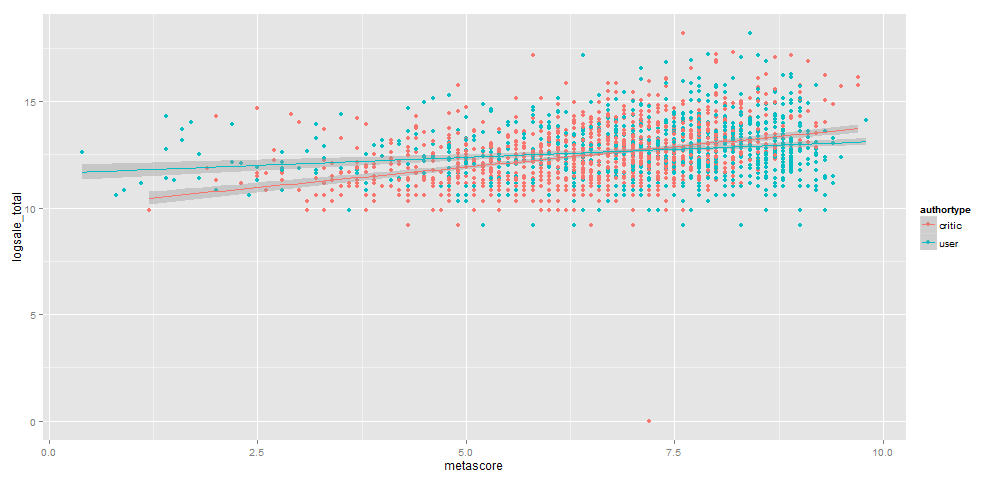
\includegraphics[width=\linewidth]{game_metascore_vs_totalsales}
\caption{metascores vs total lifetime sales}
\label{fig:metascore_totsale}
\end{figure}

\begin{figure}[tbph]
\centering
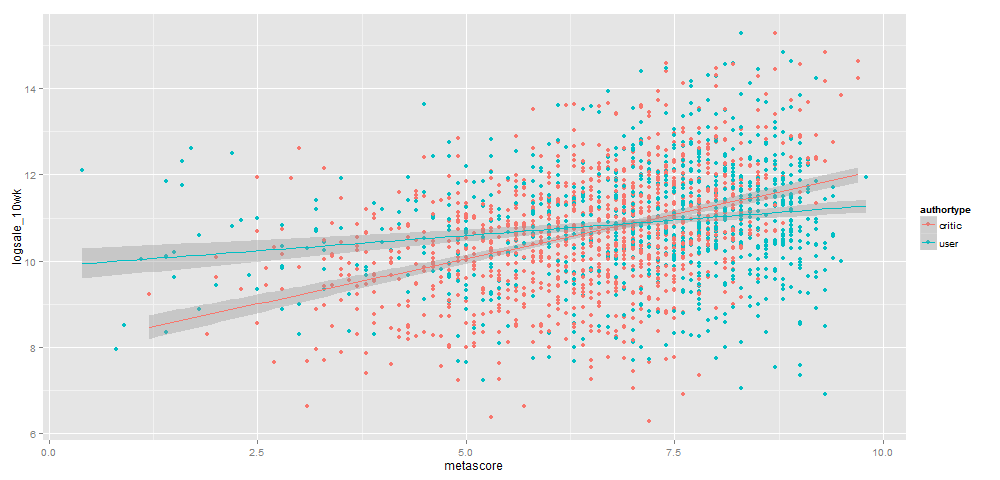
\includegraphics[width=\linewidth]{game_metascore_vs_10wksales}
\caption{metascores vs sum of first 10 week sales}
\label{fig:metascore_10wksale}
\end{figure}

\begin{figure}[tbph]
\centering
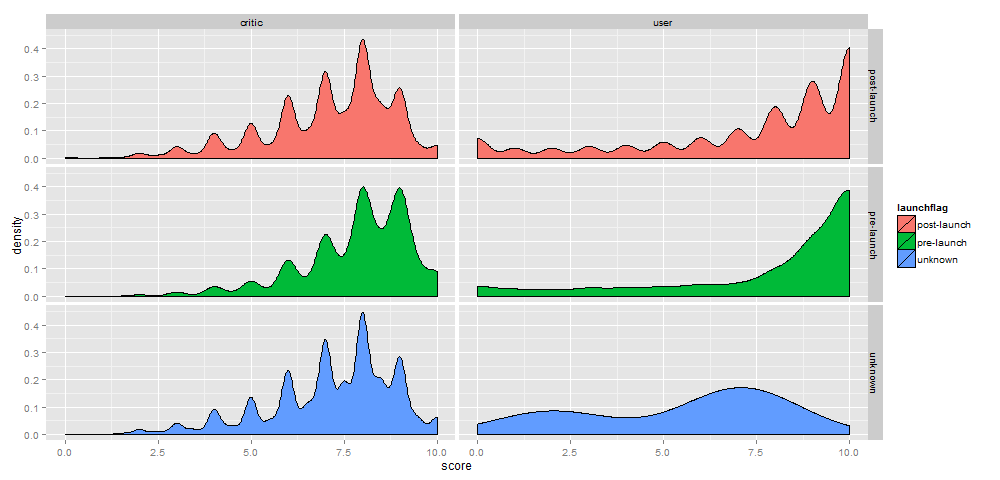
\includegraphics[width=\linewidth]{./review_score_timing_distribution}
\caption{distribution of review scores by review time from launch (unknown means review was not tagged with a date)}
\label{fig:review_score_timing_distribution}
\end{figure}

\begin{figure}[tbph]
\centering
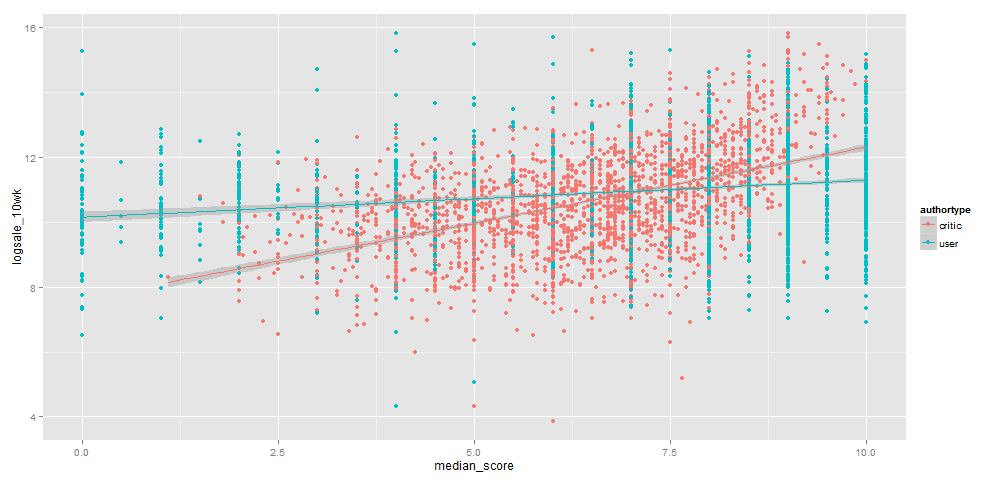
\includegraphics[width=\linewidth]{./sales_10wk_vs_medianscore}
\caption{total sales over first 10 weeks vs median score}
\label{fig:sales_10wk_vs_medianscore}
\end{figure}

\begin{figure}[tbph]
\centering
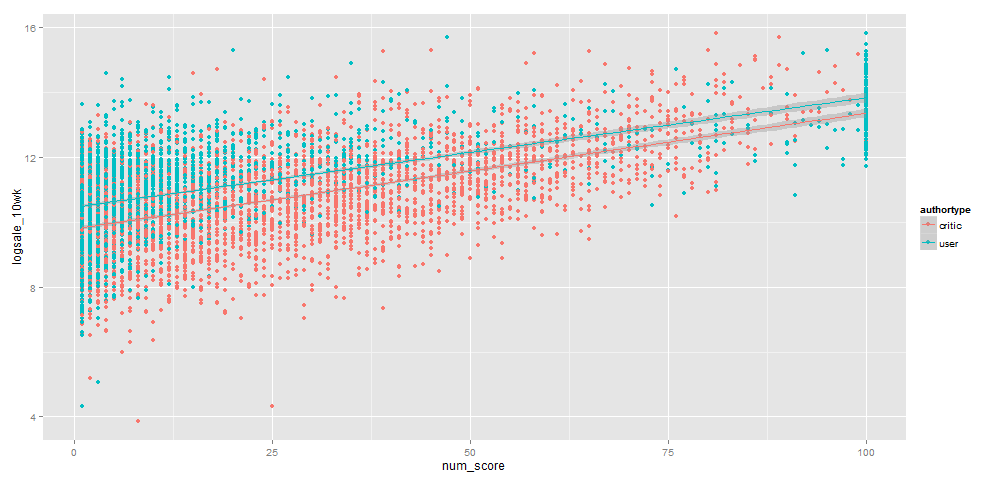
\includegraphics[width=\linewidth]{./sales_10wk_vs_reviewnum}
\caption{total sales over first 10 weeks vs number of reviews}
\label{fig:sales_10wk_vs_reviewnum}
\end{figure}

\begin{figure}[tbph]
\centering
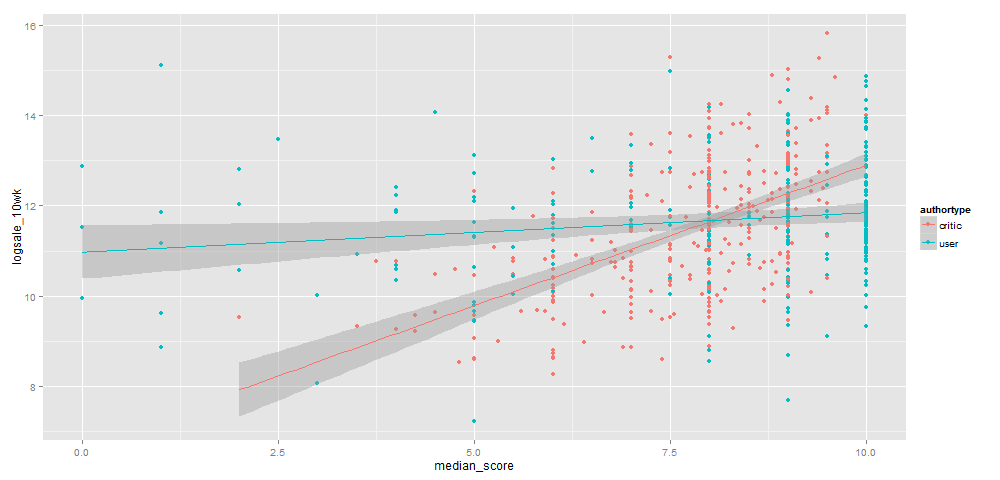
\includegraphics[width=\linewidth]{./sales_10wk_vs_medianscore_pre10}
\caption{total sales over first 10 weeks vs median score using only reviews in 10 weeks prior to week of game launch}
\label{fig:sales_10wk_vs_medianscore_pre10}
\end{figure}

\begin{figure}[tbph]
\centering
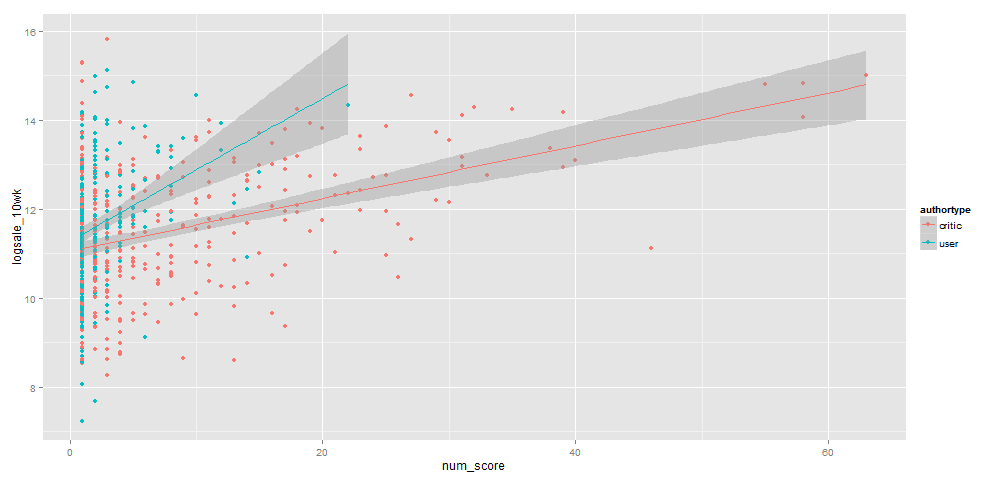
\includegraphics[width=\linewidth]{./sales_10wk_vs_numscore_pre10}
\caption{total sales over first 10 weeks vs number of reviews using only reviews in 10 weeks prior to week of game launch}
\label{fig:sales_10wk_vs_reviewnum_pre10}
\end{figure}

\begin{figure}[tbph]
\centering
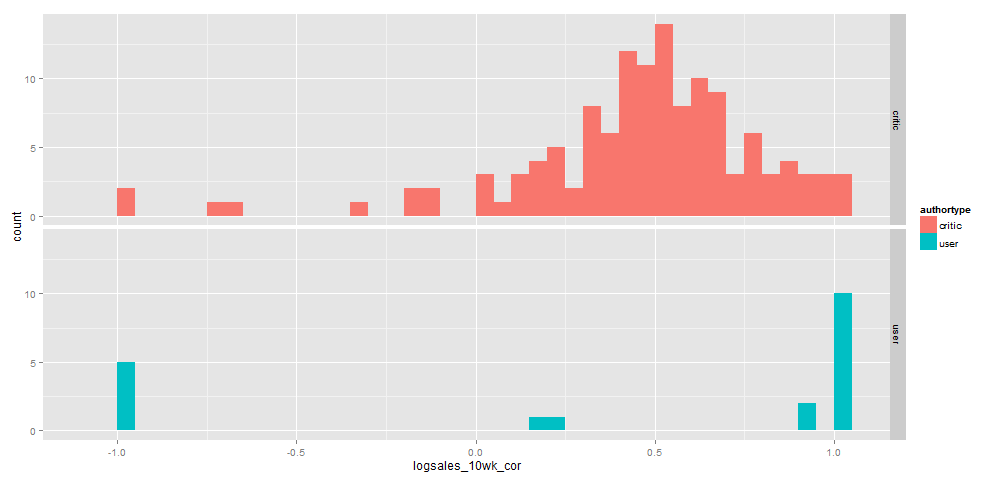
\includegraphics[width=\linewidth]{./correlation_10wk_sales_all}
\caption{histogram of correlation between reviewer scores and game 10week sales for all reviewers}
\label{fig:corr_10wksales_all}
\end{figure}

\begin{figure}[tbph]
\centering
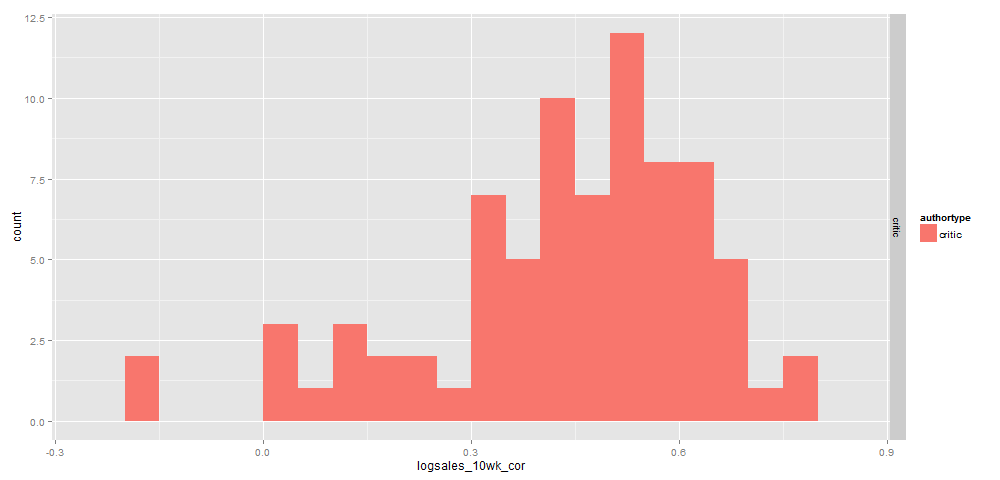
\includegraphics[width=\linewidth]{./correlation_10wk_sales_over10reviews}
\caption{histogram of correlation between reviewer scores and game 10week sales for reviewers with over 10 reviews}
\label{fig:corr_10wksales_over10}
\end{figure}


\section{Introduction}
relate product ratings to sales

- are professionals more or less useful than novices?

- what differentiates these groups?

- what does this tell us about social media practices and game purchasing/consumption?


- use classification on text to differentiate

- linear regression on scores to predict

- statistical causal analysis for deeper prediction data

\section{Related Work}
Gilbert on status \cite{gilbert2012phrases}. Gilbert on stock market \cite{gilbert2010widespread}.

Predicting future w/social media data \cite{asur2010predicting}

Predict book sales from blog discussions.

\section{Methodology}

\subsection{Corpus Collection}
We used the python Scrapy package\footnote{http://scrapy.org/} to scrape all user and critic reviews for videogames from the Metacritic website\footnote{http://www.metacritic.com/}. For every game we collected the following information: console (the hardware the game software was made for), title, publisher (company responsible for distributing the game), developer (studio responsible for making the game), release date, current metascore, current average user score, genre (according to Metacritic), and ESRB rating (age-appropriateness rating). Note that some titles may appear on multiple consoles. We treat these as separate games as they reach potentially different audiences and may vary in their implementation. From every game we also collected all user and critic reviews, including their text, review score, time of review, and a flag indicating whether the review came from a user or critic. Metacritic converts critic review scores from many formats (such as letter grade, 0-10 range, 0-100 range) into a 0-100 score. User reviews are limited to a 0-10 score range. For comparison we divide all critic scores by 10 to have all reviews on a [0-10] scale. \textbf{Metacritic only provides summary excerpts from critic reviews and we limited ourselves to this text to make review length more comparable between users and critics. Our final corpus consists of 182,036 reviews: 126,570 from critics and 55,466 from users. Of these, 81,288 critic and 6 user reviews lacked review date time stamps. These were excluded from our time-series based analyses.}

For sales data we scraped information from the VGChartz website\footnote{http://www.vgchartz.com/}. VGChartz tracks game weekly, annual, and lifetime sales data from a variety of outlets and is primarily targeted toward sales of games in the United States. Their data is most accurate for console games (rather than computer or mobile phone), so we limit ourselves to examining the following consoles: Sony's PlayStation 3 (PS3), PlayStation Portable (PSP) and Vita; Nintendo's Wii, DS, and 3DS; and Microsoft's Xbox360. These consoles are considered to make up the current ?generation? of videogame hardware and are the primary game console distribution platforms. For weekly data VGChartz typically only records the first 10 weeks of game sales, and so our time series analysis is limited to these weeks. \textbf{Of the 8475 games we have weekly sales data for, 8306 have 10 weeks of sales data, while only 1140 have the 11th week for data.}

\subsection{Analytic Models}\todo{rename!}
Our analysis involved three components: (1) predicting lifetime game sales, (2) predicting weekly game sales, and (3) identifying key words relating reviews to reviewers, review scores, and consoles described. To predict lifetime sales data we constructed a robust linear regression model for logged lifetime game sales based on median review scores using R's MASS package\footnote{http://cran.r-project.org/web/packages/MASS/}.

\textbf{Of the 3839 games with United States lifetime sales data, 3402, had at least one matching review based on game console and title.} We used a conservative approach of only keeping exact game title matches without manipulating titles (e.g. using lowercase versions or removing punctuation). In our case it is better to have a slightly smaller dataset than misattribute review scores to different sales.

We predicted weekly game sales data over the first 10 weeks of available information. Reviews and sales data were aligned to be based on weeks since release. Reviews were binned into weekly periods based on time since the release of the game. For example, all reviews within 7 days of the game's stated release date (for that console) were binned into the first week. To assess whether reviews had predictive power over the weekly time series we performed a vector autoregressive analysis. Vector autoregressive models are commonly used in econometrics to assess the predictive power of relationships between time series. Here we examine whether weekly average review scores are predictive of game weekly sales.

For the predictive task we logged all sales data to ensure normality. Review scores are provided on a week by week basis, but need not occur during every week the game has sales data. To interpolate data we first compute the running average review score at each week we have reviews. Thus, if we have reviews of 3 and 9 on the first and third weeks, the first week running average is 3 and the third week is 6. We interpolated across missing weeks by propagating forward the most recent running average score. This mimics how Metacritic website users would see the scores displayed, showing only the current running average score without accounting for future changes. In the above example the second week's interpolated score is 3. One limitation is that Metacritic uses an unweighted average for user scores (as we are), but weights critic scores. Our goal was to predict sales without knowing a priori which reviewers or critics may have greater weight, justifying this choice. For our analysis we examined two conditions: (1) averaging review scores across all games; (2) averaging review scores grouping together critics or users separately across all games. In both cases we averaged weekly sales data to date across games. A limitation of this approach is losing game-specific differentiations in predictive power - in the future we would like to explore per-game sales prediction.

We used the augmented Dickey-Fuller unit root test to test time series stationarity and found these conditions were met for running average review score, running number of reviews, and weekly logged sales data. Thus no additional differencing or controls were necessary to use this data in the predictive task. We only employ lags of 1 or 2 weeks as our sales data is limited to a 10 week period.

Our analysis of review text examined the predictive power of review text words to: (1) distinguish reviewers as critics or users; (2) predict review score; and (3) distinguish game consoles being described. We prepared our review texts using several standard methods performed in text analysis using the R programming language packages tm\footnote{http://cran.r-project.org/web/packages/tm/} and topicmodels\footnote{http://cran.r-project.org/web/packages/topicmodels/}. We removed whitespace, punctuation, numbers not part of words, and common English words (known as stopwords). All text was lowercased and stemmed to group together repeated use of similar words. We tokenized these documents into single words, requiring words be at least 3 letters long and appear in at least 10 documents. \textbf{After constructing a full corpus of 83,185 terms we removed the most sparse terms to produce a set of 2,608 terms.}

We also employed python's pattern package\footnote{http://www.clips.ua.ac.be/pages/pattern} to analyze review text sentiment. For every review text we parse the text into sentences, compute per-word sentiment (both polarity and subjectivity) and compute the per-review mean, median, and maximum sentiment values. Subjectivity values measure to what extent a text conveys an opinion. Polarity values estimate that valence as positive or negative. While we used these values to accompany the score-based prediction tasks below (in the place of score) we found they provide little additional information, and so these results will not be reported in detail.

All prediction tasks were performed using R's glmnet package\footnote{http://cran.r-project.org/web/packages/glmnet/} for generalized linear models. These models account for collinearity of terms (their frequent appearance together altering relative importance) and can control for sparsity (relative infrequency of terms). Controlling collinearity is important to prevent overweighting words that often appear together. Account for sparsity enables the model to exclude terms with little predictive power, yielding a smaller and more interpretable set of results.

Our three tasks map into different classification and regression problems. We treat user and critic distinction as a binary classification task, using binomial regression. Score prediction was modeled as a regression task using a Gaussian response model. Game console classification was treated as a multi-class classification problem using a multinomial model. Understanding review texts by console can distinguish what traits are seen as unique to a console and provide further insight into how website viewers are presented with information on different game properties. As videogames are often known for having strong ?fanboy? cultures attached to particular consoles we expect to see some variance in how they review games and potentially compare these to other games or consoles.


\section{Results}

\subsection{Corpus Overview}
Before describing results on our prediction tasks it is important to understand the characteristics of the review and sales corpuses we collected. Metacritic users are not necessarily representative of the opinions of all those interested in videogames and it is not apparent a priori how they behave compared to the critics whose reviews are featured on the site.
Users and critics show clear differences in review score attribution (Figure \ref{fig:revscore_console}). Critics tend to provide reviews distributed more tightly around a mean of 7.2 and median 7.5 score, while users show more variation with a mean 7.4 and median 9.0 score. A Wilcoxon test found these differences to be significant (p $< 0.001$). Also note that users favor providing higher scores than critics, but are the only ones likely to provide low review scores.
Intuitively these results make sense. Critics are often under threat of blacklist for providing low review scores and have a reputation to preserve by not consistently giving high review scores. Game distributors are also unlikely to provide reviewers with free game copies for review if they anticipate low ratings, while critics are unlikely to review low profile and low quality titles. These factors combine to skew critics towards reviewing games generally favorably without providing overly positive reviews. Users, in contrast, are most likely to review when a game provided a great or terrible experience. As Metacritic is a major game review outlet reviewers are likely to provide high scores to games they enjoyed, while attacking games they found poor quality or a waste of money.

\begin{figure}[tbph]
\centering
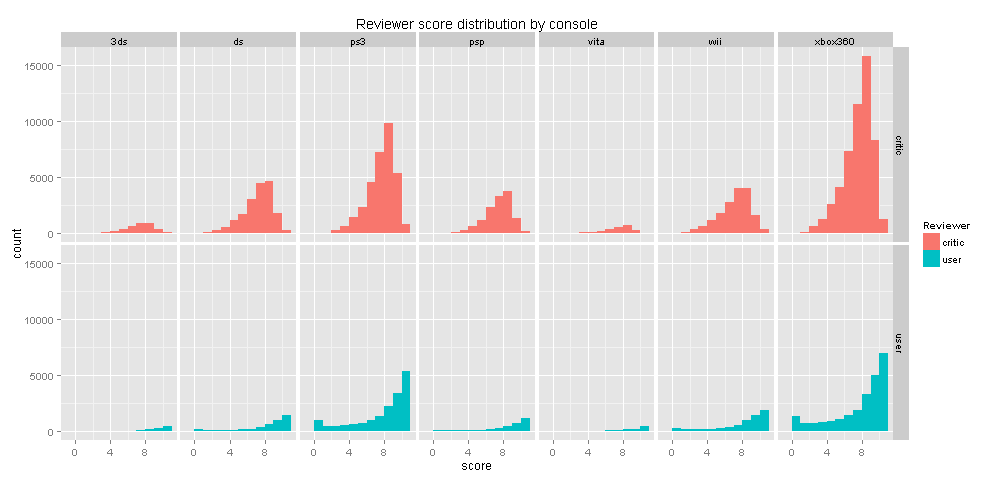
\includegraphics[width=\linewidth]{./review_score_hist}
\caption{review score distribution by console}
\label{fig:revscore_console}
\end{figure}


Reviewers and critics also show different levels of subjectivity and polarity in reviews (Figures \ref{fig:revpol_density}, \ref{fig:revpol_console} and \ref{fig:revsubj_console}). Critics show slightly greater levels of subjectivity and polarity in their reviews (Wilcoxon test; p $< 0.001$ for both). These differences are slight (mean polarity of 0.498 for critics and 0.472 for users; mean subjectivity of 0.143 for critics and 0.144 for users) yet show a general trend towards mildly subjective and positive reviews. As review scores tend to be skewed toward high values this trend is not surprising. Maximum and median polarity within texts showed similar trends.

As might be expected, critic reviews are less likely to show a direct subjective opinion. One limitation of this interpretation is that critic texts were limited to summaries and thus may not reflect the intended valence of the review, but a revised summary meant to convey factual information for the purposes of featuring on Metacritic. That critics show a greater average polarity is surprising and worth further exploration. One possible explanation is that reviewers need to provide text that drives consumer opinion, whereas users may simply provide factual information in many reviews (except those that are highly polarized). These results may also reflect limitations of our sentiment analysis itself and merit further investigation.

%\missingfigure{review polarity density} \label{fig:revpol_density}

\begin{figure}[tbph]
\centering
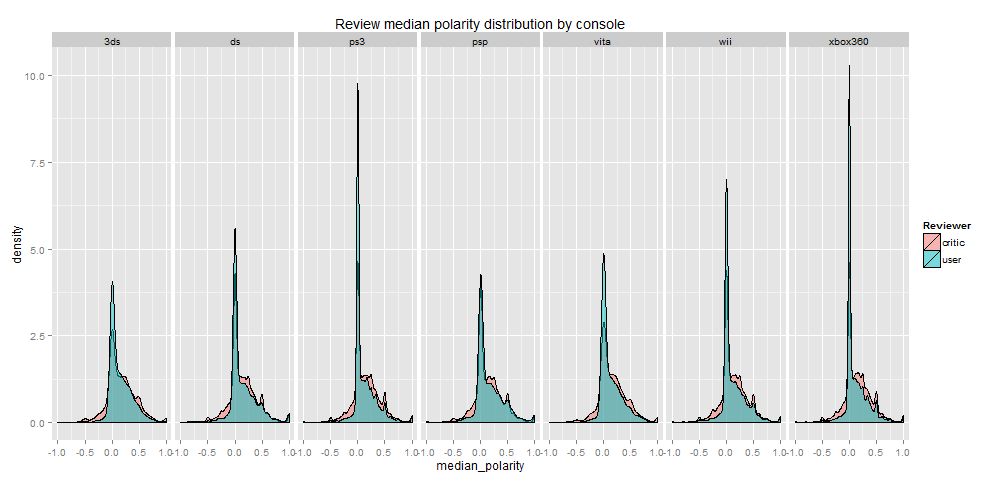
\includegraphics[width=\linewidth]{./review_polarity}
\caption{review polarity density by console comparing reviewer type}
\label{fig:revpol_density}
\end{figure}




\begin{figure}[tbph]
\centering
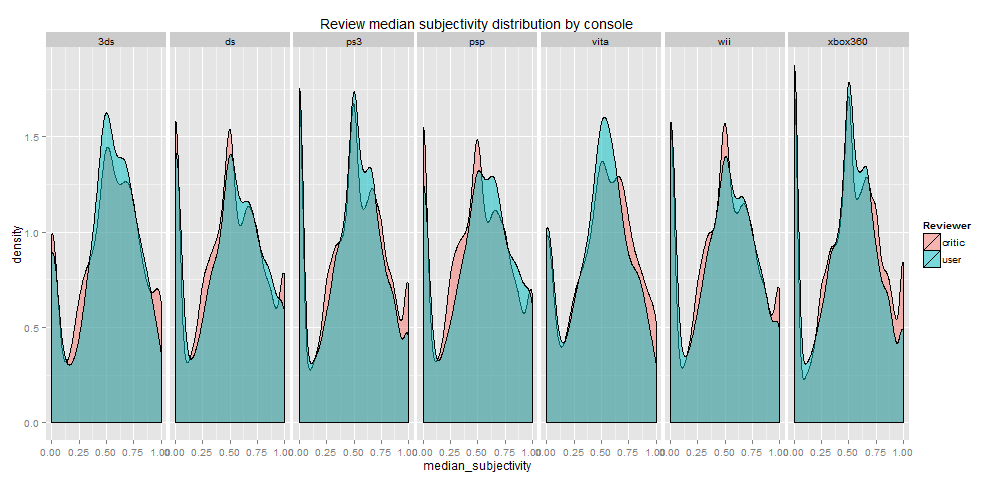
\includegraphics[width=\linewidth]{./review_subjectivity}
\caption{review subjectivity density by console comparing reviewer type}
\label{fig:revpol_subjectivity}
\end{figure}

\subsection{Lifetime Sales Prediction}
We used a linear model to predict mean lifetime sales for each game. While linear models may have limited predictive power for nonlinear relationships they also afford direct interpretation useful to analysts employing the results. Our model considered three factors: median review score, number of reviews, and the author of the review. Review scores and number show clear relationships to the lifetime sales of a game (Figure \ref{fig:lifesale_revnum} and \ref{fig:lifesale_revscore}).

\begin{figure}[tbph]
\centering
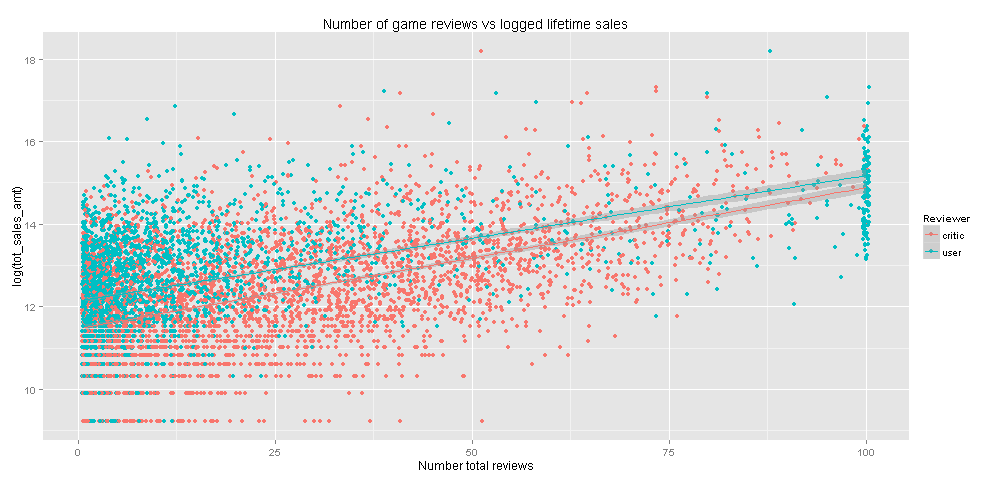
\includegraphics[width=\linewidth]{./sales_total_vs_reviewnum}
\caption{lifetime sales vs number of reviews}
\label{fig:lifesale_revnum}
\end{figure}

\begin{figure}[tbph]
\centering
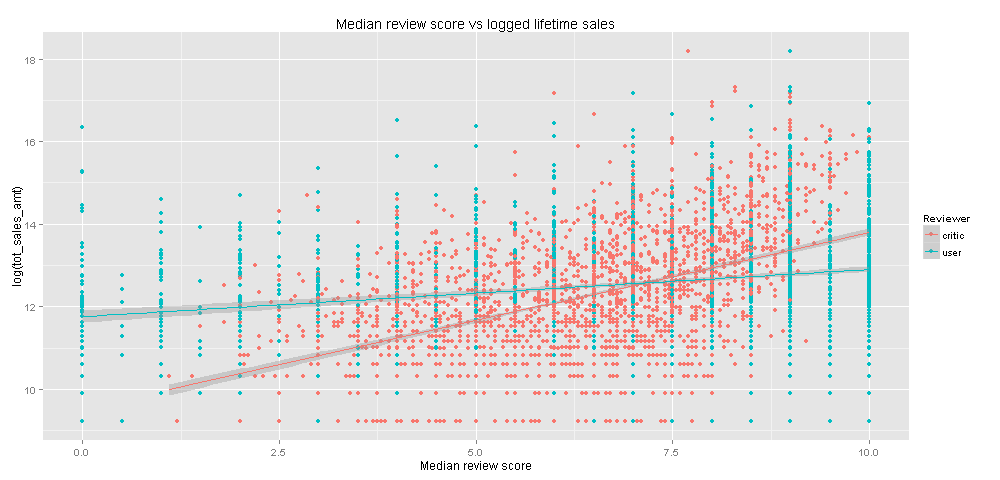
\includegraphics[width=\linewidth]{./sales_total_vs_medianscore}
\caption{lifetime sales vs median review score}
\label{fig:lifesale_revscore}
\end{figure}



\textbf{Of the 6,661 unique games with review data and 3,839 USA region sales data games 3,402 matched by a concatenation of game name and platform.}

\begin{figure}[tbph]
\centering
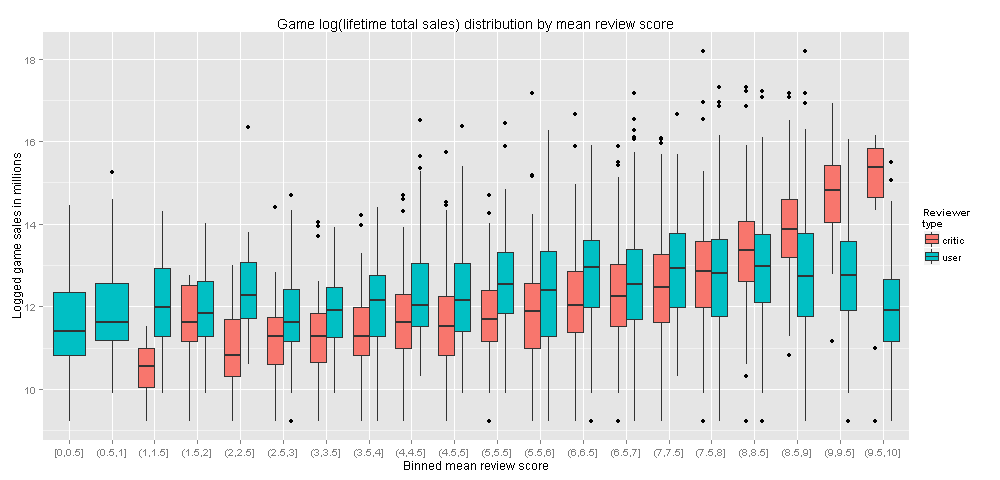
\includegraphics[width=\linewidth]{./sales_total_vs_scorebin}
\caption{lifetime sales vs binned review scores}
\label{fig:lifesale_revscore_boxplot}
\end{figure}


Anecdotally many have claimed that a rise over a metascore of 90 leads to a substantial boost to game sales. Our data supports this notion although the range of relevance is broader (Figure \ref{fig:lifesale_revscore_boxplot}). User scores do not show a clear relationship to sales: increasing mean user review score does not appear to relate to any substantial gain in scores. By contrast, critic review scores show a clear increasing relationship, starting around scores above 60 but becoming most prominent for scores above 80. While the [95-100] category has only 12 critic reviews and thus is of dubious predictive value, the [85-90] and [90-95] categories consist of 177 and 73 reviews and thus of greater predictive merit.

We built three robust regression models to predict logged total sales: mean review score and number of reviews from users only, the same from critics only, and the same from both types of users with a fourth factor accounting for reviewer type (overall). Table \ref{tab:sales_lm} summarizes our results.

\missingfigure{table of betavals and porportions of variance}\label{tab:sales_lm}

Relative importance was measured using the lmg metric measuring how important each of the predictive variables are. It averages the $R^2$ contributions of each variable over all possible orderings of factors. Overall, critic scores and number of reviews provide the greatest predictive power for game total sales.

While critic scores and number of reviews have roughly equal relative importance, user reviews are accounted for almost entirely by their volume. Given the distributions seen above this makes sense: games that have many user reviews are rare, but enjoy strong sales on average. For a game to have many user reviews requires many users to have played the game and been motivated to review the game. From the previous distributions of review scores we would expect these reviewers to (mostly) give positive scores, thus the fact that they are writing a score at all is indicative of what that score will be. Playing the game typically means a user has purchased the game, thus further entangling with sales. While direct causality cannot be read off from these results it is clear that the amount of attention users or critics devote to a game is indicative of its level of sales success. Future work should explore more sophisticated features for predicting sales such as reviews in the weeks prior to launch, number of reviews in the first weeks of sales (not just overall), or volume of previews. Twitter, Facebook, and Youtube and other media consumption information (not necessarily reviews) may be important gauges of broad consumer interest that complements the more devoted group of Metacritic user reviewers.

\subsection{Weekly Sales Prediction}
Weekly average scores show relative stability over the first 10 weeks of a game's life, while number of reviews grows steadily (Figures \ref{fig:running_score_vs_wkidx} and \ref{fig:running_number_vs_wkidx}). We examined three different vector autoregressive models to predict game sales information on: average overall score from both users and critics and running net number of reviews; solely user scores and number of reviews; and using solely critic scores and number of reviews. For each model we considered four variants: predicting either weekly sales or running total sales by either average score or number of reviews. Overall running number of reviews was predictive of weekly sales at a lag of one week, but no other variations on this model showed significant results. Weekly sales were also predictive of number of reviews at one week. Thus, the running number of reviews predicts sales one week into the future, but these sales also influence incoming reviews. Intuitively, games that have high scores are likely to have many purchase them, with these purchases in turn driving (other things being equal) more reviews.

\todo{probably cut these figures and section}
\missingfigure{average score vs weeks since launch}\label{fig:running_score_vs_wkidx}

\missingfigure{average score vs weeks since launch}\label{fig:running_number_vs_wkidx}

Considering user data two models were significant: predicting weekly sales from number of reviews and predicting running sales from number of reviews. In both cases the one week lag model was significantly predictive in both directions. User number of reviews predicts sales into the next week, but this relationship goes both ways (as above). At a lag of two weeks, number of reviews predict sales without being predicted by sales two weeks earlier. Thus the number (but not score) of user reviews are a leading indicator of future sales two weeks into the future.

Critic running number of reviews were predictive of both weekly sales and running total sales. At a lag of one week critic number of reviews predicts weekly sales, but is not predicted by prior weekly sales. Critic number of reviews also predicted running total sales at lags of one and two weeks. Critic reviews were not predicted by sales from the prior week, but were related to sales from two weeks prior.

Combined these results suggest an intuitive explanation: user review volume is tied to purchasing behavior, while critic review volume is indicative of future success. Larger user review volume is intuitively related to sales as reviewing typically implies previous purchase. Larger critic review volume likely ties to a number of factors that also explain increased sales. More critics reviewing a game reflects the relative prominence of that game and also increases the prominence of that game by providing information on it at major news outlets. As critic reviews are typically positive being reviewer is generally a sign game quality. In addition, large numbers of critics receiving and committing to reviewing a game likely indicates a strong marketing push behind the game with a publisher able to garner the attention of many critics.

\subsection{Review Text Classification}
Our previous analyses show reviews are predictive of sales to some extent. But what aspects of reviews distinguish them, particularly in terms of the words used? We explored this question by using review text in a bag of words model to differentiate reviews by their reviewer type, score assigned, and console described. Understanding these text-level differences can enable better prediction of what characteristics distinguish critic reviews in content from user reviews, what qualities reviewers describe when distinguishing high and low quality games, and how different consoles are implicitly described through their games. Overall our penalized regression models achieved substantial accuracy gains of 37-43\% over baseline random choices and 27-33\% over a frequency-based naive classification approach. A random baseline predicts each class with equal frequency. The frequency-based naive baseline predicts each class proportionate to its overall distribution in the dataset and accounts for the uneven sizes of our categories. The score regression model had a mean squared error of 2.934 and mean absolute error of 1.27. Thus, the model could predict score with an average error of roughly 1.27 points on a 10 point scale.

\missingfigure{classification accuracy values}

Our penalized regression models were able to effectively capture distinguishing features of texts with a vocabulary limited to a set of approximately 2600 terms. The penalized model removed relatively few terms for the user vs critic classification (121) and score regression (28) tasks, but removed more terms (typically 300-600) in the multiclass classification tasks (Table 2). Subdividing into more categories leads to fewer terms applying to a category and thus a smaller set of these terms is needed to distinguish that category. Below we review general trends in the terms given large weights by these predictive models.

\subsection{Users vs Critics}
Users were recognizable by slang terms and references to gaming culture and reviews. We report term coefficients in parenthesis next to terms and show word clouds of some of the most representative words to help understand these analysis. As words were stemmed we have included completions of the stems in parentheses to help interpretation.

Slang terms included phrases such as ``wtf'' (3.29), ``imo'' (4.57), ``lol'' (2.82), and ``meh'' (2.06). References to gaming culture often mentioned the culture of reviewing and purchasing: ``bought'' (1.80), ``review'' (1.73), ``opinion'' (1.48), ``bias'' (2.59), ``metacrit(ic)'' (2.99), ``gamestop'' (3.30), ``ign'' (1.75). Gamestop is a major game distribution store chain and IGN is a major game-related news and gameplay website. Users were also characterized by referring to specific features of playing games: ``fanboy'' (1.29), ``wife'' (2.64), ``server'' (1.38), ``lagg(y)'' (1.25), and ``beta'' (1.70). Servers, lag, and beta all refer to common aspects of networked online play.

Critics were most recognizable by their use of month names in reviews, followed by references to purchasing and holidays along with gameplay feature descriptors. References to game features included descriptions of gameplay perspective - ``firstperson'' (0.85) and ``thirdperson'' (1.06) - as well as gameplay style - ``roleplay'' (1.32) and ``actionpack(ed)'' (1.23).
Combined, these results paint a picture of critics taking a more professional role of identifying purchase products and describing their features, while users relate their games to broader consumption practices and gaming culture. Users are free to reference particular game distributors or review biases in ways critics cannot. Compared to critics, users typically relate games back to playing behavior, experiences, and culture. In part these results help understand the power of critic review scores to predict sales better than user review scores. Critics describe games in a way to guide purchasing decisions, while users are more likely to reflect on a game in their play practices and purchasing experiences with relatively little information to help understand the product features themselves.

\subsection{Score Regression}
Positive scores typically associated with relatively generic praise terms, but also showed a set of terms used as refutations of negative perceptions of others. Specifically, several terms referenced low evaluation by others: ``underr(ated)'' (0.58), ``troll'' (0.63), ``hater'' (0.80), and ``skeptic'' (0.52). These terms refer to outsiders (such as ``trolls'', ``haters'' and ``skeptics'') seeing the game as low value (``underrating''). ``addict(ive)'' (0.50) also shows a fairly strong positive association with score. In gaming culture addictive play is often used as a term of praise and this notion was clearly captured by our model.

Negative scores referenced the economic value of a game and quality of the gameplay, aside more common negative phrases. Purchasing behavior and value were prominent indicators of low score: ``bought'' (0.22), ``wast(e) [of money]'' (1.27), ``overpr(iced)'' (0.89), ``advertis(ed/ement)'' (0.84), ``tie(-)in'' (0.67) and ``ripoff'' (0.75). Gameplay was also referenced negatively as ``unplay(able)'' (1.58), ``broken'' (0.72), ``tedious'' (0.61), or a ``rehash'' (0.69).

Beyond the domain-generic aspects of praise and condemnation, the score regression model reveals specific ways gaming reviews demonstrate valuation. Gameplay features show most commonly in references to lack of functionality. Value is often construed instead in terms of a lack of wasting money, with references to being an overlooked game.

For reference we provide additional results on score prediction when employing only the subset of reviews from users or critics in the appendix (Table 8). Qualitatively the results are similar but show differential use of several key terms and foci. The user rating only regression task achieved a mean squared error of 5.05 and mean average error of 1.70; the critic model had a mean squared error of 1.74 and mean average error of 1.01. Thus, critic reviews? word use is more closely tied to provided scores than user reviews. This likely reflects the pressure on critics to provide a coherent message to readers. Wider overall variance in user score (Figure 1) also means the user text model must be accurate over a broader score range, allowing the error to potentially be larger.

\subsection{Console Classification}
While our model achieved moderately high accuracy for console classification, the terms used are primarily clustered around specific games, hardware, and companies involved with the platform. As shown in the Appendix in Table 7, the vast majority of high-weight terms are based on the specific games or companies associated with a game console. We have highlighted the three major consoles - Wii, Playstation 3 (PS3), and Xbox 360 - although the results were qualitatively similar across the other consoles. The primary differences for other platforms relate to the nature of mobile and handheld hardware against at-home consoles.

Terms positively associated with the Wii were specific to Nintendo (who manufactures the hardware), major franchises on the platform (Kirby, Zelda, Metroid, Pokemon, Mario Galaxy), and other consoles produced by Nintendo (NES, SNES, GBA). Other Nintendo hardware is to be expected as the Wii offers a service to digitally distribute games from previous hardware iterations. By contrast, most of the negative terms (associated with a text describing any console but the Wii) associate with franchises that have cross-platform releases on the PS3 and Xbox 360 but not on the Wii, such as The Elder Scrolls: Oblivion, Assassin's Creed: Brotherhood, or Fallout. Word clouds scaled by predictive coefficient magnitude for positive and negative terms of all reviews for the Wii console are shown in Figures 10 and 11 respectively.

\missingfigure{console positive term wordle}\label{fig:positive_wordle}

\missingfigure{console negative term wordle}\label{fig:negative_wordle}

Terms positively and negatively associated with both the PS3 and Xbox 360 show similar trends. Franchises and hardware positively associated with the Wii were negatively associated with both the PS3 and Xbox 360. In general the terms positively and negatively associated with the PS3 and Xbox 360 were often overlapping. These results align with the confusion matrix for each console (see Appendix Tables 3 and 4). All consoles were often misclassified for the Xbox 360, but these rates were particularly high for mistaking the PS3 or Xbox 360 for one another. The Xbox 360 makes up 42.37\% of the total number of reviews, followed by the PS3 at 27.17\% of reviews. Classification will thus be biased towards selecting one of these consoles. These results also likely reflect the relative similarity of the two consoles in terms of hardware and software available compared to other consoles used.

The general lack of more generalizable terms from these classifications is a limitation of the model we constructed. Pre-processing the data to remove these names would likely yield more general features, but at the cost of classification accuracy. While we can only speculate, the few more general terms that appeared suggest some general aspects of the games reviewers describe. The Wii was identifiable by references to terms such as ?nextgen? and ?realism?, while ?gimicki?, and ?minigame? were (negative) identifiers for the PS3 and Xbox 360. Overall these terms reinforce the notion of a conceptual divide between the Wii's emphasis on party software and family entertainment compared to the focus on realism on the PS3 and Xbox 360.

\section{Discussion}
Our analyses of game sales and reviews uncovered several primary differences between users and critics that highlight their differential roles in promoting and consuming games. Critics employ a narrow range of review scores, are less subjective but more polar in reviews, and are predictive of lifetime sales both in terms of scores assigned and volume of reviews. The number of critic reviews for a game during the first 10 weeks of sales is predictive of sales one week into the future. Critics commonly discuss sales periods and gameplay style at a feature level. Combined, these results paint a portrait of critics as dispassionate professional sources of information and key leading indicators of overall investment in game production values and marketing push. In contrast, users are more likely to give low review scores, tend to skew towards high review scores, are less polar in their reviews than critics, and are only predictive of sales by the volume of reviews provided. User number of reviews both predicts and is predicted by ongoing sales, highlighting the coupling between providing reviews and purchasing games. User reviews highlight the reviewing context of games and experience of games at home. Together these results portray user reviewers as consumers evaluating the quality of a game purchase and its relative merit for others.

Comparing users and critics we see critics as providing ?objective? facts describing games, with scores guiding initial market interest. User reviews appear to gauge the broader uptake of games by a community of players, with scores indicating the relative success or failure of a game to meet expectations, although too late to have a strong negative impact on sales of the given game (although perhaps not the franchise). Overall, users and critics provide alternative perspectives on games through their reviews, with both being relatively strongly predictive (30-37\% of variance explained) of future sales success.

\subsection{Limitations}
Our work has several important limitations both in terms of the models employed and generalization of our results. We intentionally employed linear predictive models for lifetime sales and running weekly sales. Linear models allow for easy and direct interpretation but lose the nuance in these almost certainly non-linear relationships. The bidirectional relationships we found for time series data suggest the models we used are not sufficiently sophisticated to capture the relationships of interest. Sales and reviews seem to drive one another. These complications highlight a limitation in interpreting our results: while clear relationships exist in our data they do not necessarily indicate causality and likely reflect a variety of influencing factors.

To improve these methods we need more sophisticated time series analyses - such as Granger causality analysis - and a more refined set of predictive variables. Taking mean sales and scores across all games loses a large amount of the variance in our model, washing out key differences of interest. Thus we need models that better handle predictions for multiple related time series (running weekly sales) from multiple related time series (running average scores or total number of reviews). Our combination of game data into relative time since launch prevents us from accounting for seasonal differences in sales - such as holiday sales jumps - or interactions between sales of games released at similar times. Sales can easily be hurt by prominent competitors or bolstered through cross-marketing with other games, factors we currently ignore.

The data we used potentially limits generalization based on our model. Our corpus is derived from a single website and critic reviews were limited to summary text. It is unclear whether the user/consumer reviewing patterns of users on other websites would show similar relationships as Metacritic is considered a prominent source for game review information. Perhaps the number of user reviews only matters from major outlets, while other venues have less influence on sales. Limiting critic text to summaries may have hurt the power of our models to detect any language critics employ in a full review text. Yet this is typically what users would find when seeking critic reviews. By employing summaries we maintained the interface of Metacritic, but this comes at the cost of missing the more general patterns of how critics review when presenting materials on their own venue.

Our text-based models are further hamstrung by using solely unigrams in a bag-of-words model. The prominence of terms like ?hater? as a positive association with review score highlights the role of linguistic qualifications and negations in reviews. The terms we provide are an initial foray into the space of review descriptions, but further work is needed to untangle the kinds of relationships being described. Even capturing simple adjective-noun relations would add depth and potential insight into what aspects of games reviewers describe and how they describe them.

\subsection{Applications}
The most obvious application for our work is predicting game sales from Metacritic reviews. Publishing firms can use this as a guide to forecast sales based on ongoing success to vary the resources devoted to supporting a game (particularly those with online or ongoing components). Marketers might attempt to drive user reviews in an effort to improve interest. Although we have not demonstrated a causal connection, this strategy presents itself as one worth exploring.

Review sites such as Metacritic develop ad hoc schemes for converting among multiple review systems. Employing predictive models based on score or features could potentially provide a unifying metric for game ?quality? that puts all scores on a unified scale. For game marketers and producers this can quantify the value of reviews they get when selecting potential reviewers. For reviewers, this can enable them to focus reviews on their desired features without having to conform to accepted scoring systems. Losing familiar user guides to scoring may hurt interpretability for users, but may also allow both users and critics to focus more on aspects of game features or experience without filtering these results through an arbitrary number.

\subsection{Future Work}
Several avenues are available for extending this work toward better understanding the user-critic distinction and improving the predictive models employed. Beyond improving the sophistication of the natural language processing techniques used to examine review texts we might compare users and critics from other websites or sources. Do users of different websites provide different perspectives on games? Metacritic is known as a major review center and thus likely reflects the opinions of more devoted game players. Other review sources such as Amazon may have a wider audience that is indicative of general opinions or perspectives on games. Combining these sources may uncover how users of these sites differ and have varying predictive powers. For example, more ?casual? games? sales may be better predicted by Amazon reviews while Metacritic reviews may better capture sales of more niche games. Identifying key words and phrases predictive of sales - rather than score alone - may also be an important future avenue to consider.

Critics were the best source of predictive information for lifetime sales. Metacritic claims the metascore is a valuable summary of the quality of a game. Can we construct an analogous metric for weighting critic scores based on predictive accuracy for sales data? Can we employ review and sales data to assign relative value to critics based on their use for predicting future sales? How predictive is a game's metascore for lifetime sales? Our averaged critic scores show predictive power for lifetime sales but how this compares to metascores remains unexplored. We can even imagine constructing a ?meta-metacritic? that combines the assessments of multiple review websites into a single metric predictive of game sales. Such a rating might convey how useful information from different websites is for assessing a game and predicting future success.

Given the predictive power of the sheer number of user reviews for sales we might consider alternative ways to gauge this form of grassroots interest. Amazon or other major online retail sources? reviews may reflect more general market trends and levels of interest. As most reviews happen within the first two to three weeks of a game's release we could potentially gather further information on the ?pulse? of interest using real-time information from Twitter, Facebook, and similar social venues. Do these sources provide complementary information? Can they enable better real-time prediction? Trends in Google search behavior (available from Google trends) or advertising Youtube videos may also provide useful supplemental predictive power.

Our analyses were limited to the first 10 weeks of game sales and excluded personal computer and mobile distribution platforms (such as Apple's app store or Google's Android marketplace). These venues hold promise for additional aspects of user reviews tied to the long-term success of a game. Console games traditionally have the bulk of sales early in release followed by a long tail of reduced sales. Yet some titles are ``evergreen'' and continue to have comparatively strong sales over months or years of their life. User reviews in particular may be predictive of these titles as users often provide reviews much longer after a game's release compared to critic reviews that tend to cluster around release. Mobile and personal computer markets are also widely considered to be domains where this evergreen phenomenon is more common, making them valuable sources of information to consider. Expanding our analyses to these more longitudinal domains has great potential for improving our sales prediction methods and potentially identifying game traits users describe when choosing to play a game that is older.

\section{Acknowledgments}
thank Eric Gilbert for class, Joshua Johnson and Kevin Terraciano for help on project.

\bibliographystyle{aaai}
\bibliography{icwsm13}

\end{document}
